\documentclass{standalone}
\usepackage{tikz}

\begin{document}
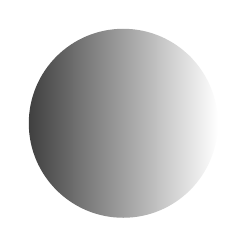
\begin{tikzpicture}[scale=2]
    % Draw the central circle (white)
    \fill[white] (0,0) circle (0.15);

    % Draw the radial lines (black)
    \foreach \i in {0,45,...,315} {
        \draw[thick, black] (0,0) -- (\i:0.6);
    }

    % Draw the outer circle (white)
    \draw[white] (0,0) circle (0.6);

    % Add some shading to give it a more realistic look
    \shade[left color=white, right color=gray!50!black] (0,0) circle (0.15);
    \shade[left color=gray!50!black, right color=white] (0,0) circle (0.6);
\end{tikzpicture}
\end{document}